\documentclass{icmmcm}
%\usepackage[dvips]{graphicx}  % For importing graphics for use with
                              % dvips.
\usepackage[pdftex]{graphics} % For importing graphics for use with
                              % pdftex or pdflatex.
\usepackage[numbers]{natbib}

%%% Sample ICM/MCM Contest Submission
%%%
%%% C.M. Connelly <cmc@math.hmc.edu>
%%%   for the Department of Mathematics, Harvey Mudd College
%%%   Copyright 2003. 


%%% ---------------
%%% Local Command and Environment Definitions

%%% If you have any local command or environment definitions, put them
%%% here or in a separate style file that you load with \usepackage.

% \newtheorem declarations
\newtheorem{Theo1}{Theorem}
\newtheorem{Theo2}{Theorem}[section]
\newtheorem{Lemma}[Theo2]{Lemma}
% Each of the above defines a new theorem environment.
% Multiple theorems can be done in the same environment.
% Theo2's number is defined by the subsection it's in.
% Theo3 uses the same numbering counter and numbering system as
% Theo2 (that's the meaning of [Theo2]).


%%% TeX has an excellent hyphenation algorithm, but sometimes it
%%% gets confused and needs some help.
%%%
%%% For words that only occur once or twice, you can insert hints
%%% directly into your text, as in
%%%
%%%    our data\-base system is one of the most complex ever devised
%%%
%%% For words that you use a lot, and that seem to keep ending up at
%%% the end of a line, however, inserting the hints each time gets to
%%% be a drag.  You can use the \hyphenation command  to globally tell
%%% TeX where to hyphenate words it can't figure out on its own.

\hyphenation{white-space}

%%% End Local Command and Environment Definitions
%%% ---------------


%%% ---------------
%%% Title Block

\title{A Hexagonal Model of Repeater Coordination}

%%% Which contest are you taking part in?  (Just one!)

\contest{ICM}

%%% The question you answered.  (Again, just the one.)

\question{B}

%%% Your Contest Team Control Number
\team{15118}


%%% A normal document would specify the author's name (and possibly
%%% their affiliation or other information) in an \author command.
%%% Because the ICM/MCM Contest rules specify that the names of the
%%% team members, their advisor, and their institution should not
%%% appear anywhere in the report, do *not* define an \author command.

%%% Defining the \date command is optional.  If you leave it blank,
%%% your document will include the date that the file is typeset, in
%%% the form  ``Month dd, yyyy''.

% \date{}

%%% End Title Block
%%% ---------------

\begin{document}

%%% ---------------
%%% Summary

\begin{summary}
  The contest rules specify that you should include a one-page summary
  of your report.  This page appears before the rest of the report,
  and will have a special header attached to it that takes up the top
  2.5" of the page.

  By typing your summary inside a \texttt{summary} environment, \TeX\ will
  handle the formatting of that page correctly, including leaving
  space at the top of the page and not numbering the page.
  
  It will also reset the page numbers so that the first page of your
  report is labeled correctly.
  
  What should you put here?  Basically, you want a brief restatement
  of the problem followed by a largely \emph{non-technical}
  description of what you've done.  Try to avoid using mathematical
  notation.
  
  You probably want to write a few paragraphs, around half to
  two-thirds of a page.

  For 2009, the COMAP folks said the following about the summary:
  \begin{quotation}
    The summary is a very important part of your MCM paper. The
    judges place considerable weight on the summary, and winning
    papers are sometimes distinguished from other papers based on
    the quality of the summary. To write a good summary, imagine
    that a reader may choose whether to read the body of the paper
    based on your summary. Thus, a summary should clearly describe
    your approach to the problem and, most prominently, what your
    most important conclusions were. The summary should inspire a
    reader to learn the details of your work.  Your concise
    presentation of the summary should inspire a reader to learn
    the details of your work. Summaries that are mere restatements
    of the contest problem, or are a cut-and-paste boilerplate
    from the Introduction are generally considered to be
    weak.

To Summarize:
\begin{description}
\item[Restatement Clarification of the Problem]
---

\item[Assumptions with Rationale/Justification]---emphasize those
  assumptions that bear on the problem. List clearly all variables
  used in your model.

\item[Model Design and justification for type model used/developed.]

\item[Model Testing and Sensitivity Analysis, including error
  analysis, etc.]

\item[Discuss strengths and weakness to your model or approach.]

\item[Provide algorithms] in words, figures, or flow charts (as a step
  by step algorithmic approach) for all computer codes developed.
\end{description}
 \citep{comap-mcm-rules}
\end{quotation}

\end{summary}
 
%%% End Summary
%%% ---------------

%%% ---------------
%%% Print Title Block, Contents, et al.

\maketitle
\tableofcontents

%%% Uncomment the following lines by deleting the % sign
%%% if you have figures or tables in your report:
\listoffigures
\listoftables  
 
%%% End Print Title Block, Contents, et al.
%%% ---------------

\section{Introduction}%
\label{sec:introduction}


In the Very High Frequency (VHF) communication system, the signal by itself cannot go much farther than the line-of-sight, because it travels as a straight line while the earth surface is curved, thereby limiting the range that two VHF users can directly communicate. The usage of repeaters can solve this problem by amplifying the weak signal it receives and, to avoid self-interference, transmits at a slightly different frequency but in a stronger transmitting power, hence extending the range of communication significanly. However, the two repeaters might interfere with each other and interrupt the comminucation for both of them. To solve this problem, we need to design a coordination system of repeaters to avoid the interference, either by placing them their locations or using sufficiently different frequencies. Further, we are given the technology of CCTCS or Private Line (PL) for a repeater to distinguish two signals with the same frequency but different PL tones, therefore reducing the number of repeaters needed at a place.

The goal to approach this problem is to design a repeater coordination system that minimizes the number of repeaters but is meanwhile capable to accommodate 1,000 people \emph{simultaneously} (meaning that \emph{after} we know where those 500 pairs of people live, we design a model to allow them to communicate to each other). Our approach to this problem is to design a mathematical model to simulate a uniform distribution of people and determine how many repeaters are required for each region.

\noindent -------------------- TODO:
the history and context of the problem,
and your work and results.  Your introduction should be more detailed
and technical than your summary.  You may also want to include an
outline of your report, along the lines of
\begin{quotation}
  In Section~1 we give our definitions and notation. Section~2
  describes our numerical experiments\ldots{}..
  
  We prove our main result, Theorem~6, in Section~5\ldots{}.
\end{quotation}
Of course you would replace the numbers in that example with
appropriate \verb|\ref| commands pointing to the correct
\verb|\label|s in your source.\\
-----------------------

\section{Givens}
\begin{enumerate}
\item We are given that Blah
\item We are given the usage of Private Line (PL).
\item The study area is flat and of the 40-mile radius.
\item The number of simultaneous users is 1,000.
\item The range of frequencies is 3 MHz (3,000 kHz), ranging from 145 to 148 MHz.
\item The offset is $\Delta(f)$ = 600 kHz.
\item We have 54 PL tones in total.
\end{enumerate}

\section{Assumptions}

\begin{enumerate}
\item A repeater can serve multiple usages for the same frequency, providing that the PL tones are different. If a repeater senses at least two signal with the same frequency and same PL tone, then the communication collapse and this mishap should not happen at at point of the system.
\item The interference is discrete. If two repeaters are closer than $R$, the range of each repeater, then they interfere each other. On the other hand, if the distance is more than $R$, then the two repeaters are independent. If, however, the distance is approxiamtely $R$, we assume that they can either connected (not intefere) with each other. A reason for this is that the real usage of a chain of repeaters called ``reverse splits'' use this (TODO: explain).  

\item Assume that the range of repeaters is fixed in this problem. According to (TODO: find some website that is more reliable than Wiki), the range depends on the antenna's height as follows:
$$R\text{(mile)}=\sqrt{1.5\times A_f},$$
where $A_f$ is the antenna's height in foot. This equation is deviant when the are is mountainous, which we will explore in a later section. The typical heights of the antenna is about 15 to 50 feet, corresponding to the range R of 5 to 10 miles.  
\item From the design of using 600 kHz as an offset frequency, we assume that 600 kHz is a threshold. The difference of frequencies lower than this threshould should interfere. (TODO: verify this!)
\item The distribution of people is a variable. However, we assume that once the people live, they are static. That is, we can think of those people as stations communicating to one another but not moving.
\item To avoid the ambiguity when one person, say A, wants to communicate to B but the voice also travels to C and D. We assume that A can overcome this ambiguity by indicating a code when starting the conversation, such as ``Call B. This is A. Line number 4,''  so that C and D can stop listening and that B knows which line to contact back to A.
\end{enumerate}
\section{Model Design}

\subsection{Setup}
\begin{enumerate}
\item The main part is about location. We need to configure a good location, and the PL tones and 3 different sets of frequencies can help reducing the number of repeaters later. (explain why. TODO)
\item We introduce the hexagonal-coordinate system. TODO: explain why we can use hexagons to approximate circles, and how the radius of 40 miles compared to $R$ of 10 miles, plays a role in this model.

Figure~\ref{fig:hex_coor} is an example of our definition of the hexagonal coordinate. Notice that it needs not fit into the circle. The $y-$axis is $60^\circ$ to the $x-$axis. Note that the point $(-1,-1)$ is in the circle where as the point $(1,1)$ is not, even though the origin of the circle is at $(0,0).$
\begin{figure}[ht]
\begin{center}
\scalebox{0.3}{\includegraphics{hex_coor}}
\end{center}
\caption[Hexagonal Coordinate System]{Hexagonal Coordinate System.\label{hex_coor}}%
\label{fig:hex_coor}
\end{figure}

\item We generate a distribution of of people in two types: uniform and cluster (a city model).
\item For any pair of people, find the shortest distance $s$ between the two and keep track the multiple possible paths. Add one to the nodes it travels through, meaning that that point needs an additional repeater for this path. Ultimately, these two people will choose only one way to communicate (over than this is a waste), so we need to divide the number of repeaters added from the previous step by the total number of possible paths. This method will keep the distribution of possible paths accurately while having the total number of repeaters added repeaters equal to $s$ (since for each path we add $s$ for the account of newly added repeaters.) (TODO: simplify this!)
\item MORE ASSUMPTION: we assume that the repeaters locate at integer coordinates only!
\item Also we need to mention that we use python, I think.
\end{enumerate}
\subsection{Theorems}
\begin{Theo1}
For a given point $C$, of all the paths from point $A$ to point $B$, the number of repeaters needed at point $C$ is equivalently increased by 
$$\frac{\text{nPaths}(A,C)\cdot \text{nPaths}(C,B)}{\text{nPaths}(A,B)},$$
where $\text{nPaths}(X,Y)$ is a function that returns the number of possible \emph{shortest} paths from $X$ to $Y$, which is given in Theorem 2.
\end{Theo1}
{\bf Proof.}
It follows from the principle of counting:
\begin{align*} \text{The weight for additional repeaters at C}
&=\frac{\text{The number of paths from A to B via C}}{\text{The number of paths from A to B}}\\
&=\frac{\text{nPaths}(A,C)\cdot \text{nPaths}(C,B)}{\text{nPaths}(A,B)}.
\end{align*}\hfill $\Box$


\begin{Theo1}
Given two points $A$ and $B$ in the hexagonal-coordinate system. Let $\Delta x$ be subtraction of the $x$-component of $B$ by that of $A$ and $\Delta y$ for $y$-component. The number of \emph{shortest} paths from point $A$ to $B$ is given as follows:

\[ \text{nPaths}(A,B) = 
\begin{cases} 
  \dbinom{|\Delta x+\Delta y|}{ |\Delta x|}, & {\emph \rm if~} \Delta x\Delta y\geq 0;\\

  \dbinom{\max{\left(|\Delta x|,|\Delta y|\right)}}{\min\left(|\Delta x|,|\Delta y|\right)}, & {\emph \rm otherwise,}\\
\end{cases}
\]
and by a shortest path we mean the sum of lengths of its subpaths, not the Pythagorean distance.
%$$\text{nPaths}(A,C)=if(deltaX*deltaY >= 0):
%       return choose(abs(deltaX + deltaY),abs(deltaX))
%    else:
%      smaller = min(abs(deltaX),abs(deltaY))
%    bigger = min(abs(deltaX),abs(deltaY))
%   return choose(bigger,smaller)$$

\end{Theo1}
{\bf Proof.}
(The Principle of Extreme.) We will use the principle of extreme to prove this. In each step, from the hexagonal coordinate, the point can move to an adjacent point only in these following three forms (recall Figure~\ref{hex_coor}):
\begin{enumerate}
\item[(X)] Move in the $x$ direction, either towards the more potitive or negative end.
\item[(Y)] Move in the $y$ direction, either towards the more potitive or negative end.
\item[(Z)] Move in the $x$ direction in one way (more positve or more negative), and, at the same time move in $y$ direction in the opposite way (more negetive or more positive, respectively). This move is a diagonal movement.
\end{enumerate}
We will show that at most \emph{two} forms of those three forms are made when we seek the shortest possible paths (can be more than one path) from one point in the hexagonal coordinate to another point. 
Consider the extreme case: the case where path is shortest. This case exists by the Well Ordering Principle. Suppose to contrary that we can those three forms of movement each at least once. Note that the movement in either the $x$ or the $y$ direction, or both, should draw the starting point towards the destination. For otherwise we could move the point back one step and that indicated that we have wasted two steps, a contradiction to the assumption that the path we are considering is the shortest one. So, each move will draw the initial point to the destination, either in the $x$ (by (X)) or the $y$ (by (Y)) direction, or both (by (Z)). Next, because we use three forms at least once, we can combine one move by (X) and another one by (Y) to become just one move. Notice that no matter what order of steps, we yield the same result. Thus, this combining of (X) and (Y) is possible and so we could have saved one more step, a contradiction to the assumption that this path is the shortest one. Now we can conclude that we can use at most two forms.

Then, the rest of the proof follows from the fomula of the number of ways going two direction from the initial point towards the destination. If, for example, we need to use (X) form $a$ times and use (Y) form $b$ times. The way to count this is $\tbinom{a+b}{a}$ ways, by selecting which steps out of $a+b$ that we will choose (X). The rest of the proof is similar, but for the case for (X) and (Z), and (Y) and (Z), we need to check which axis is achieved first when we apply (Z) repeatedly. (TODO: simplify this whole page!)
\hfill $\Box$

\begin{Theo1}
For the level of hexagons of $n$, the number of areas is
$$6n^2.$$
\end{Theo1}
{\bf Proof.}
There are six triangle subsectors of a hexagon. For each sector, the number of triangle is $1, 3, 5, \ldots, (2n-1)$. Each sector represents one area. Thus, the total number of areas is
$$6(1+ 3+ 5+\cdots+ (2n-1))=6n^2.$$\hfill $\Box$

%%=================NEW SECTION
\section{Model Testing}

Take a look at an example below, where we put the city into our hexagonal coordinate (Both X and Y range from -3 to 3):
\begin{table}[htbp]
  \begin{center}
    \begin{tabular}{@{}c|rrrrrrr@{}} \toprule
X and Y  	&-3 	&-2 		&-1		&0		&1		&2		&3\\ \midrule   
3&15.53	&34.87	&36.03	&32.00	&0.00	&0.00	&0.00    \\ 
2&36.73	&76.12	&104.57	&81.22	&43.00	&0.00	&0.00	\\
1&37.13	&94.27	&137.75	&138.05	&91.57	&54.00	&0.00	\\
0&31.0	&82.1	&134.47	&\textbf{158.42}	&140.13	&83.07	&35.00	\\
-1&0.00	&51.0	&113.25	&137.35	&145.05	&111.92	&39.12	\\
-2&0.00	&0.00	&49.00	&89.37	&99.00	&92.42	&46.47	\\
-3&0.00	&0.00	&0.00	&33.00	&32.15	&36.18	&27.72	\\
 \bottomrule	
    \end{tabular}
  \end{center}
  \caption[A Distribution of Repeaters for a Uniform Distribution of People]{The table of the number of conversations (reflecting the number of repeaters) at each point. The number of people is 1000. The level of hexagons is 3.}
  \label{tab:uniform}
\end{table}

From Table~\ref{tab:uniform}, we have the total number of repeaters of 2,780. Hence, the actual number of repeaters needed (with help of PL tones) is 51.48. As there are $6\times(3^2)=54$ regions as well, the number of repeaters needed per 1 PL tone per 1 location is 0.953. This can be done easily since we have 3 frequency sets to serve. One concern is the service at the peak: the middle (point $(0,0)$). The original number of repeaters needed is 158.42. By using PL tones, we have the avearge of $2.93$ users using one PL tone. Again, this use can be accommadated by 3 different sets of frequencies. Thus, in this case, the total number of repeaters required is 51.48, approximately \boxed{52 \text{ repeaters}} , each holding differnt 54 PL tones.

%Figure~\ref{sample1} is an example of repeater coordination.
%\begin{figure}[!hbtp]
%\makebox[\textwidth]{\framebox[8cm]{\rule{0pt}{8cm}}}
%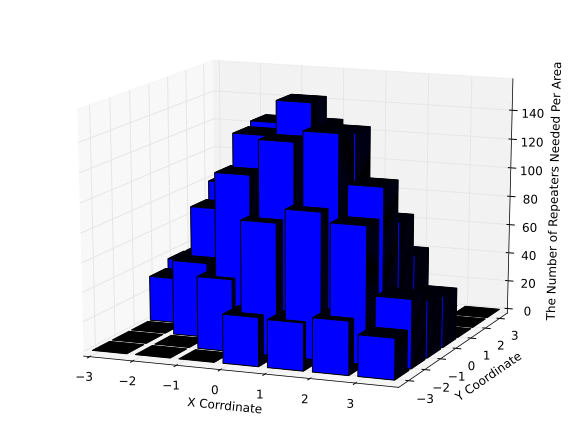
\includegraphics[width=7cm]{sample1.png}
%\caption{Sample 1 Distribution of Repeaters (Maximum at the Middle).\label{white}}
%\end{figure}

Figure~\ref{fig:sample1} is an example of repeater coordination.
\begin{figure}[ht]
\begin{center}
\scalebox{0.6}{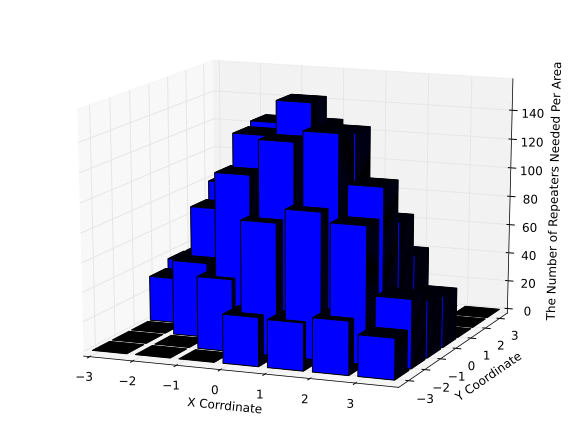
\includegraphics{sample1}}
\end{center}
\caption[A Distribution of Repeaters for a Uniform People Distribution]{A Distribution of Repeaters (Maximum at the Middle).\label{sample1}}%
\label{fig:sample1}
\end{figure}

\section{Sensitivity Analysis And Error Analysis}
We do several cases and find the standard deviation. Also, we can try to plot a function of the minimum number of repeaters depending on the number of people. If we were to plot this graph, there would be a limit point in which no repeater coordination can serve that number of simultaneous users.

Figure~\ref{sensitivity} represents the data test for sensitivity.
\begin{figure}[ht]
\begin{center}
\scalebox{0.6}{\includegraphics{sensitivity}}
\end{center}
\caption[Sensitivity of the Model]{Sensitivity Analysis with a Change in the Number of People.\label{sensitivity}}%
\label{fig:sensitivity}
\end{figure}
The reduced Chi-square value for this data set is 0.496. This is a good value, indicating that the number of repeaters is proportional to the number people, although the negative deviation this reduced Chi-square from 1.000 suggests that the line fits the data too well. The cause of this happening might be because we generate an almost completely randomized distribution of people. In the reaility, though, the distribution will be be as uniform as our model. For this particular data, the number of repeaters needed for 1,000 people is \boxed{51.7\pm 0.7 \text{ units.}}
\section{Comments}
Strength: accuracy of counting!
Weakness: need not be at the node.

\section{The Model Algorithm}
Long!

\section{Adapted Models}
\subsection{The population of 10,000 people}
In this case, I think the center of the town will have a lot of problems because we don't have enough PL tones and sets of frequencies to distinquish to coming signals. Our program reports the number of repeaters needed at the center as large as 1377, corresponding to the actual required number of repeaters of 514 with help of PL tones, and so each location needs approximately 10 sets of frequencies. We only have 3. There are many ways to solve this, such as extending the range of frequency, extending the area, and increasing the number of PL tones.

\subsection{Mountainous Area}
For the area that is mountainous, the range $R$ of each repeater is decreased. Therefore, we need more chains of repeaters in order to accomplish the same task. The level of haxagons will increase. If we set it to five, here is a result when we have 1,000 people:

Figure~\ref{mountainous} is an example of repeater coordination for a mountainous area.
\begin{figure}[ht]
\begin{center}
\scalebox{0.6}{\includegraphics{mountainous}}
\end{center}
\caption[A Distribution of Repeaters for a Mountainous Area]{Distribution of Repeaters for a Mountainous Area (Maximum at the Middle).\label{mountainous}}
\label{fig:an-eps-graphic}
\end{figure}
Total is 4831.0. The repeaters per 1PL tone is  is 89.46 (This value reflects the total number of repeaters needed). Per one location is 0.596. We have 3 sets of frequencies, so this case will be easy to deal with. The peak at the middle is about 158.42. The number of sets of frequencies needed is 
$$\frac{158.42}{(\text{The number of areas})(\text{The number of PL tones})},$$
which is 
$$\frac{158.42}{(6\cdot 5^2)(54)}=\boxed {0.020.}$$
This value means that we can use only one frequency even at the middle of the town.  Although this data suggests that we need to use more repeaters (as much as 90 repeaters, as opposed to 52 repeaters), we perform better in terms of avoiding frequency interference.

\subsection{A Non-Uniform Distribution}
In this section, we will explore cases where the distribution of people is not uniform anymore. People live together, more closely in the capital. This adaptation in the model might reflect upon this reality better. In our model, we use the Normal Distribution that has the center at some point, say the point that is of scale 0.2 on both $x$- and $y$-axes considering the possible range. We use the standard deviation of 0.5, not too big to let the point fall outside the scope. Below is the result:

\begin{table}[htbp]
  \begin{center}
    \begin{tabular}{@{}c|rrrrrrr@{}} \toprule
X and Y  	&-3 	&-2 		&-1		&0		&1		&2		&3\\ \midrule    
3&78.23	&41.65	&39.38	&24.00	&0.00	&0.00	&0.00 \\
2&100.78	&99.27	&65.13	&46.98	&15.00	&0.00	&0.00	\\
1&130.98	&133.83	&130.20	&83.75	&43.30	&19.00	&0.00	\\
0&107.00	&167.32	&\textbf{172.68}	&161.28	&89.97	&40.73	&22.00	\\
-1&0.00	&97.00	&153.37	&158.77	&134.52	&68.23	&33.60	\\
-2&0.00	&0.00	&89.00	&151.90	&118.47	&89.75	&41.27	\\
-3&0.00	&0.00	&0.00	&100.00	&113.43	&84.47	&62.75	\\

 \bottomrule	
    \end{tabular}
  \end{center}
  \caption[A Distribution of Repeaters for a Non-Uniform Distribution of People]{The table of the number of conversations (reflecting the number of repeaters) at each point. The number of people is 1000. The level of hexagons is 3.}
  \label{tab:non-uniform}
\end{table}

Figure~\ref{skew} represents the data test for sensitivity. From the ~\ref{tab:non-uniform}, we have that the peak is at point $(0,-1)$. With help of PL tones, the number of repeaters needed for this case is $\frac{172.68}{54}=3.19.$ This means that the 3 sets of frequencies is not enough and we might have some inteference as we can use at most 3 sets of frequencies at this point.
\begin{figure}[ht]
\begin{center}
\scalebox{0.6}{\includegraphics{skew}}
\end{center}
\caption[A Distribution of Repeaters for a Non-Uniform Distribution of People]{Non-Uniform Distribution of People And Its Effect on the Number of Repeaters Needed.\label{skew}}%
\label{fig:skew}
\end{figure}
\section{Conclusion}

All's well that ends well.


%%% ---------------
%%% Bibliography

%\nocite{*}   %%% Include everything in the thesis.bib file.  Be
             %%% careful---some journals and fields expect you to only
             %%% include references for materials that you have
             %%% actually cited in your paper, others allow you to
             %%% include materials you used as ``background'' without
             %%% actually citing specific pages or passages.

%%% Feel free to choose any bibliography style you like.
\bibliographystyle{plainnat}
%%% The filename (without the bib extension) of your bibliography file.
\bibliography{icmmcm}

\end{document}



